%============================================================
\section{Nombre: Circulo de fuego.} \label{hab.CirFue}
\subsection{Descripción}
El enemigo se rodea a sí mismo con fuego, este ataque sera usado cuando el jugador se encuentre a una distancia corta del enemigo. El fuego que rodea al enemigo durara un periodo de tiempo determinado y después desaparecerá. El fuego reducirá la cantidad de vida del jugador al hacer contacto con éste. El fuego no afectara a otros objetos que no sean el jugador. Mientras esta habilidad se encuentre activa, el enemigo no recibirá daño por parte del jugador.
\subsection{Portador}
Itzpápalotl (ver apartado \ref{per:itzpapalotl}),  Mictlantecutli (ver apartado \ref{per:mictlantecutli}). 
\subsection{Esquema}
			Ver figura \ref{fig:circuloF}.
			\begin{figure}
				\centering
				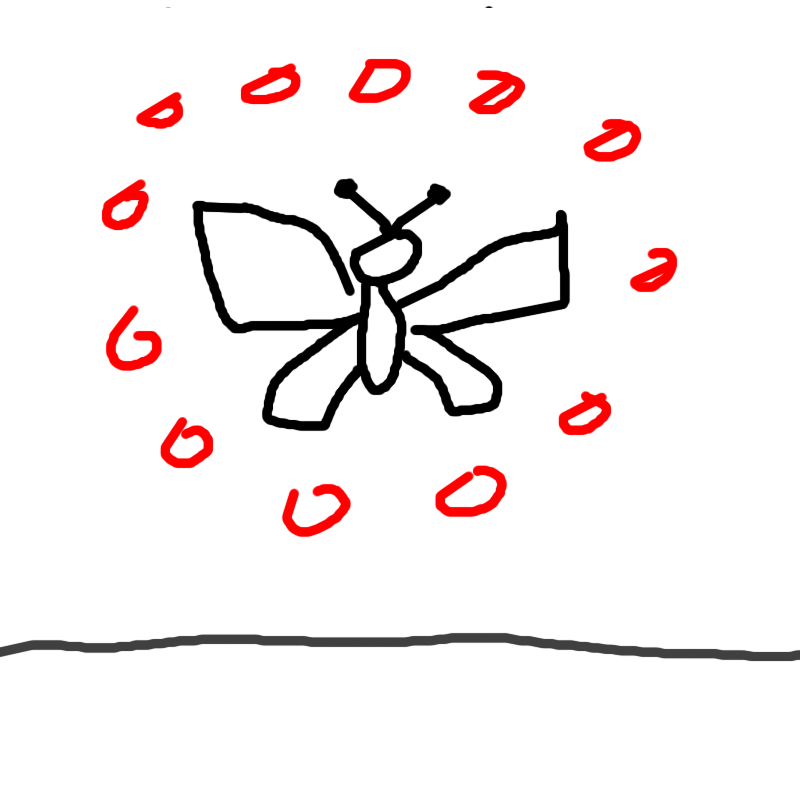
\includegraphics[height=0.2 \textheight]{Imagenes/circuloF}
				\caption{Círculo de fuego.}
				\label{fig:circuloF}
			\end{figure}
			